\documentclass{article}
\usepackage[utf8]{inputenc}
\usepackage[brazilian]{babel}
\setlength{\voffset}{0pt}
\usepackage[bottom=2cm,top=2cm,left=3cm,right=2cm]{geometry}
\usepackage{amsmath,amssymb,amsthm}
\usepackage{gensymb}
\usepackage{graphicx}
\usepackage{grffile}
\usepackage[section]{placeins}
\newcommand\tab[1][1cm]{\hspace*{#1}}

\title{EP2 - Relatório}
\author{Lucas Seiki Oshiro - 9298228\\ Marcos Vinicius do Carmo Sousa    - 9298274}

\begin {document}
\maketitle
\section{Parte 0: O Laboratório}

\section{Parte 1: O Zoológico}
Foram feitos experimentos com imagens coloridas e em tons de cinza. As funções escolhidas foram:
\begin{itemize}
	\item Colorida:
	\subitem a) $f(x,y) = (sen(x), \dfrac{sen(y) + sen(x)}{2}, sen(x)$ (Fornecida no enunciado, função de classe $C^{2}$)
	\subitem b) $f(x,y) = (sin(x), \dfrac{sin(\frac{y}{10}) + sin(\frac{x}{10})}{2}, sin(x))$ (Função de classe $C^{2}$)	
	\subitem c) $f(x,y) = (\dfrac{x}{150}, \dfrac{x}{10}$ mod $ 2, \dfrac{y}{300})$ (Função que não é de classe $C^{2}$)
	\subitem d) $f(x,y) = (\dfrac{x}{150} + \dfrac{y}{600}, \dfrac{x^{2}}{\sqrt{x^{2} + y^{2}}} * \dfrac{1}{151}, \dfrac{x}{300} + \dfrac{y}{150})$ (Função de classe $C^{2}$)
	
	\item Tons de cinza:
	\subitem e) $f(x, y) = cos(\dfrac{x}{151\pi}) + cos(\dfrac{y}{151\pi})$ (Função de classe $C^{2}$)
	\subitem f) $f(x, y) = \dfrac{x}{10}$ mod $2$ (Função que não é de classe $C^{2}$)
	\subitem g) $f(x, y) = \dfrac{x^{2}}{\sqrt{x^{2} + y^{2}}} * \dfrac{1}{151}$	(Função de classe $C^{2}$)
\end{itemize}

Os experimentos foram feitos para $k=1, 2, 3$ e $h=0.1, 0.2, 1$. O erro foi proporcional ao número $k$. No método com interpolação bilinear, as variações de $h$ não produziram efeito; já no método com interpolação bicúbica, o $h$ produziu algumas diferenças, porém, não foi possível encontrar um $h$ ótimo universal, e nem uma regra que associe o valor de $h$ a um erro maior ou menor, uma vez que cada imagem obteve um melhor resultado com um $h$ diferente.

O programa funcionou melhor para imagens em tons de cinza, isso não foi um fator de grande relevância, uma vez que as imagens encontradas foram mais.

Funções mais suaves, de classe $C^{2}$, causam menos erros, porém, se a imagem for gerada com amostragens em pontos cujo valor da função sejam muito diferentes, o programa será menos eficaz na interpolação. Prova disso é o resultado de a), que gerou erro na ordem de $26\%$, e de g), que gerou erro na ordem de $0.5\%$, na interpolação bicúbica, sendo as duas funções de ordem $C^{2}$, em imagens coloridas, com $k = 1$ e $n = 0.1$. Em contrapartida, a função c) que não é classe $C^{2}$ gerou erro de $5\%$, levemente alto (acima de experimentos com imagens reais, feitos na parte 2), para os mesmos $k$ e $h$, sendo que essa função possui grande amostragem de pontos em que a função tem valores próximos. Nota-se, assim, um comportamento melhor para as funções de classe $C^{2}$.

Comprimindo a imagem gerada pela função d) com $k = 7$, e a descomprimindo com interpolação bicúbica, $k = 7$ e $n = 1$, ocasionou erro de $3.7\%$, e fazendo o mesmo processo, porem descomprimindo 3 vezes com $k = 1$, o erro foi de $2.8\%$, portanto, o segundo método se mostrou mais eficaz. Fazendo-se o mesmo procedimento com interpolação bilinear, o segundo processo também se mostrou mais eficaz, porém, a diferença foi pouca ($38.86\%$ contra $38.8\%$)

\begin{figure}[!hbt]
	\centering
	
\includegraphics[width=0.2\linewidth]{zoologico/color4}
	\caption{Imagem gerada pela função d)}
\end{figure}

\begin{figure}[!hbt]
	\centering
	
\includegraphics[width=0.2\linewidth]{zoologico/7}
	\caption{A mesma imagem, comprimida e descomprimida com $k = 7$}
\end{figure}

\begin{figure}[!hbt]
	\centering
	
\includegraphics[width=0.2\linewidth]{zoologico/1 1 1}
	\caption{A mesma imagem, comprimida com $k=7$ e descomprimida 3 vezes com $k = 1$}
\end{figure}

\begin{figure}[!hbt]
	\centering
	
\includegraphics[width=0.2\linewidth]{zoologico/pb2}
	\caption{Imagem gerada pela função f)}
\end{figure}

\begin{figure}[!hbt]
	\centering
	
\includegraphics[width=0.2\linewidth]{zoologico/pb2decompressed}
	\caption{A mesma imagem, comprimida com $k=7$ e descomprimida com $k=7$}
\end{figure}

\newpage
\section{\newpage Parte 2: A Selva}
\begin{center}

\end{center}
	\tab Foram realizadas testes em 4 imagens diferentes, sendo duas delas efeitos em tons de cinza das outras duas.
	As imagens escolhidas foram:\\
	\begin{itemize}
		\item Lua
	\begin{figure}[!hbt]
		\centering
		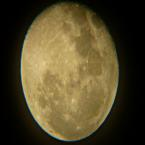
\includegraphics[width=0.2\linewidth]{imgs/lua.jpg}
		\caption{Imagem formato jpg, tamanho $p = 145$}
				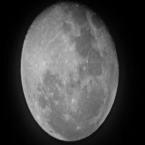
\includegraphics[width=0.2\linewidth]{imgs/lua_gray.jpg}
				\caption{Mesma imagem em tons de cinza, tamanho $p = 145$}
	\end{figure}
	
			\item Flor
			\begin{figure}[!hbt]
				\centering
				
\includegraphics[width=0.2\linewidth]{imgs/flor.jpg}
				\caption{Imagem formato jpg, tamanho $p = 145$}
				
					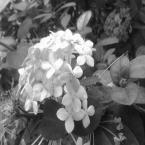
\includegraphics[width=0.2\linewidth]{imgs/flor_gray.jpg}
					\caption{Mesma imagem em tons de cinza, tamanho $p = 145$}
			\end{figure}\\
			
	\end{itemize}
	\newpage
	Conforme foi realizado na parte 1, os experimentos foram feitos com valores de $k = 1, 2, 3$ e $h = 0.1, 0.5, 1$ para os dois métodos, bilinear e bicubica.\\

		\begin{figure}[!hbt]
			\centering
			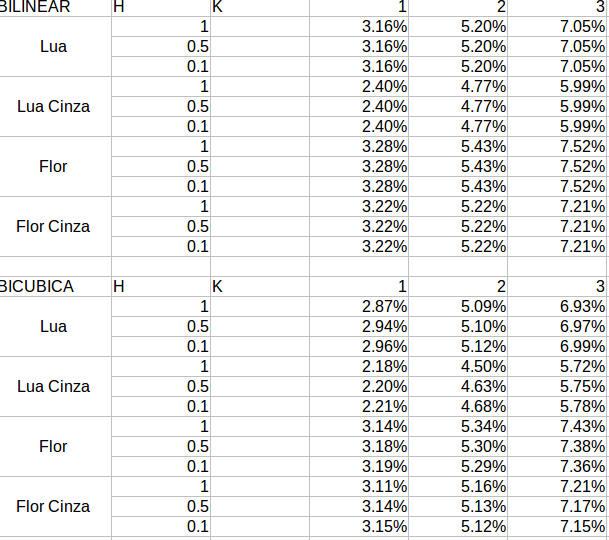
\includegraphics[width=0.7\linewidth]{imgs/erros.png}
			\caption{Tabela com os erros de cada teste}
		\end{figure}
			\tab Ao analisar o erro de cada um dos testes, é possível perceber que o erro de descompressão das imagens em tons de cinza comparado com as imagens normais, são menores sempre. Observa-se também que no método bilinear, a variação  de $h$ não altera o valor do erro, a unica referencia que se tem, é que quando aumentamos o valor de $k$, o erro cresce proporcionalmente. \\
			\tab No método de interpolação bicubica o erro varia conforme a variação de $h$, mas não há uma relação clara entre os dois. O que ocorre ainda, é a relação entre o erro e a variável $k$, quanto maior o $k$, maior o erro.\\
			\tab Realizando experimento de compressão com $k=7$ e descomprimir $3$ vezes com $k=1$ e $h=1$ a imagem da Lua, com o método bilinear, obtivemos um erro de $14.25\%$, e com o método bicubica o erro foi de $12.8\%$.\\
			Realizando agora a descompressão direta com $ k = 7 $, temos que na bilinear o erro foi de $14.29\%$, enquanto no bicubica o erro foi $14\%$. Nesse experimento realizando a descompressão em etapas, tornou-se um resultado melhor com um erro menor.
			\end{document}
